%%%%%%%%%%%%%%%%%%%%%%%%%%%%%%%%%%%%%%%%%
% Beamer Presentation
% LaTeX Template
% Version 1.0 (10/11/12)
%
% This template has been downloaded from:
% http://www.LaTeXTemplates.com
%
% License:
% CC BY-NC-SA 3.0 (http://creativecommons.org/licenses/by-nc-sa/3.0/)
%
%%%%%%%%%%%%%%%%%%%%%%%%%%%%%%%%%%%%%%%%%

%----------------------------------------------------------------------------------------
%	PACKAGES AND THEMES
%----------------------------------------------------------------------------------------

\documentclass{beamer}
%\documentclass[notes=only]{beamer} % Use this option to generate note slides

\usepackage{algorithm2e}

%\SetAlgoCaptionSeparator{.\space}
%\renewcommand\AlCapFnt{\normalfont\scshape}

\mode<presentation> {

% The Beamer class comes with a number of default slide themes
% which change the colors and layouts of slides. Below this is a list
% of all the themes, uncomment each in turn to see what they look like.

%\usetheme{default}
%\usetheme{AnnArbor}
%\usetheme{Antibes}
%\usetheme{Bergen}
%\usetheme{Berkeley}
\usetheme{Berlin}
%\usetheme{Boadilla}
%\usetheme{CambridgeUS}
%\usetheme{Copenhagen}
%\usetheme{Darmstadt}
%\usetheme{Dresden}
%\usetheme{Frankfurt}
%\usetheme{Goettingen}
%\usetheme{Hannover}
%\usetheme{Ilmenau}
%\usetheme{JuanLesPins}
%\usetheme{Luebeck}
%\usetheme{Madrid}
%\usetheme{Malmoe}
%\usetheme{Marburg}
%\usetheme{Montpellier}
%\usetheme{PaloAlto}
%\usetheme{Pittsburgh}
%\usetheme{Rochester}
%\usetheme{Singapore}
%\usetheme{Szeged}
%\usetheme{Warsaw}

% As well as themes, the Beamer class has a number of color themes
% for any slide theme. Uncomment each of these in turn to see how it
% changes the colors of your current slide theme.

%\usecolortheme{albatross}
\usecolortheme{beaver}
%\usecolortheme{beetle}
%\usecolortheme{crane}
%\usecolortheme{dolphin}
%\usecolortheme{dove}
%\usecolortheme{fly}
%\usecolortheme{lily}
%\usecolortheme{orchid}
%\usecolortheme{rose}
%\usecolortheme{seagull}
%\usecolortheme{seahorse}
%\usecolortheme{whale}
%\usecolortheme{wolverine}

%\setbeamertemplate{footline} % To remove the footer line in all slides uncomment this line
\setbeamertemplate{footline}[page number] % To replace the footer line in all slides with a simple slide count uncomment this line

\setbeamertemplate{navigation symbols}{} % To remove the navigation symbols from the bottom of all slides uncomment this line
}

\usepackage{graphicx} % Allows including images
\usepackage{booktabs} % Allows the use of \toprule, \midrule and \bottomrule in tables

%----------------------------------------------------------------------------------------
%	TITLE PAGE
%----------------------------------------------------------------------------------------

\title[A GP Approach to QoS-Aware Web Service Composition including Conditional Constraints]{A GP Approach to QoS-Aware Web Service Composition including Conditional Constraints} % The short title appears at the bottom of every slide, the full title is only on the title page

\author{Alexandre Sawczuk da Silva, Hui Ma, Mengjie Zhang} % Your name
\institute[Victoria University of Wellington] % Your institution as it will appear on the bottom of every slide, may be shorthand to save space
{
\textbf{Evolutionary Computation Research Group}\\
School of Engineering and Computer Science, Victoria University of Wellington \\ % Your institution for the title page
%\medskip
%\textit{\{Alexandre.Sawczuk.da.Silva, Hui.Ma, Mengjie.Zhang\}@ecs.vuw.ac.nz} % Your email address
}
%\date{\today} % Date, can be changed to a custom date
\date{\footnotesize \textit{IEEE Congress on Evolutionary Computation, 25-28 May 2015}}

\begin{document}

\begin{frame}
\titlepage % Print the title page as the first slide
\end{frame}

\note{Good afternoon everyone, I'm Alex and today I will talk about our paper on A GP Approach to Web service composition with conditional constraints.}

%----------------------------------------------------------------------------------------
%	PRESENTATION SLIDES
%----------------------------------------------------------------------------------------

%------------------------------------------------
\section{Motivation} % Sections can be created in order to organize your presentation into discrete blocks, all sections and subsections are automatically printed in the table of contents as an overview of the talk
\subsection{} % A subsection can be created just before a set of slides with a common theme to further break down your presentation into chunks
%------------------------------------------------

\begin{frame}
\frametitle{Introduction}
%\tableofcontents
\textbf{Service-Oriented Architecture (SOA):} Organise processes and data in reusable modules for integration into new applications.
\vfill
\centerline{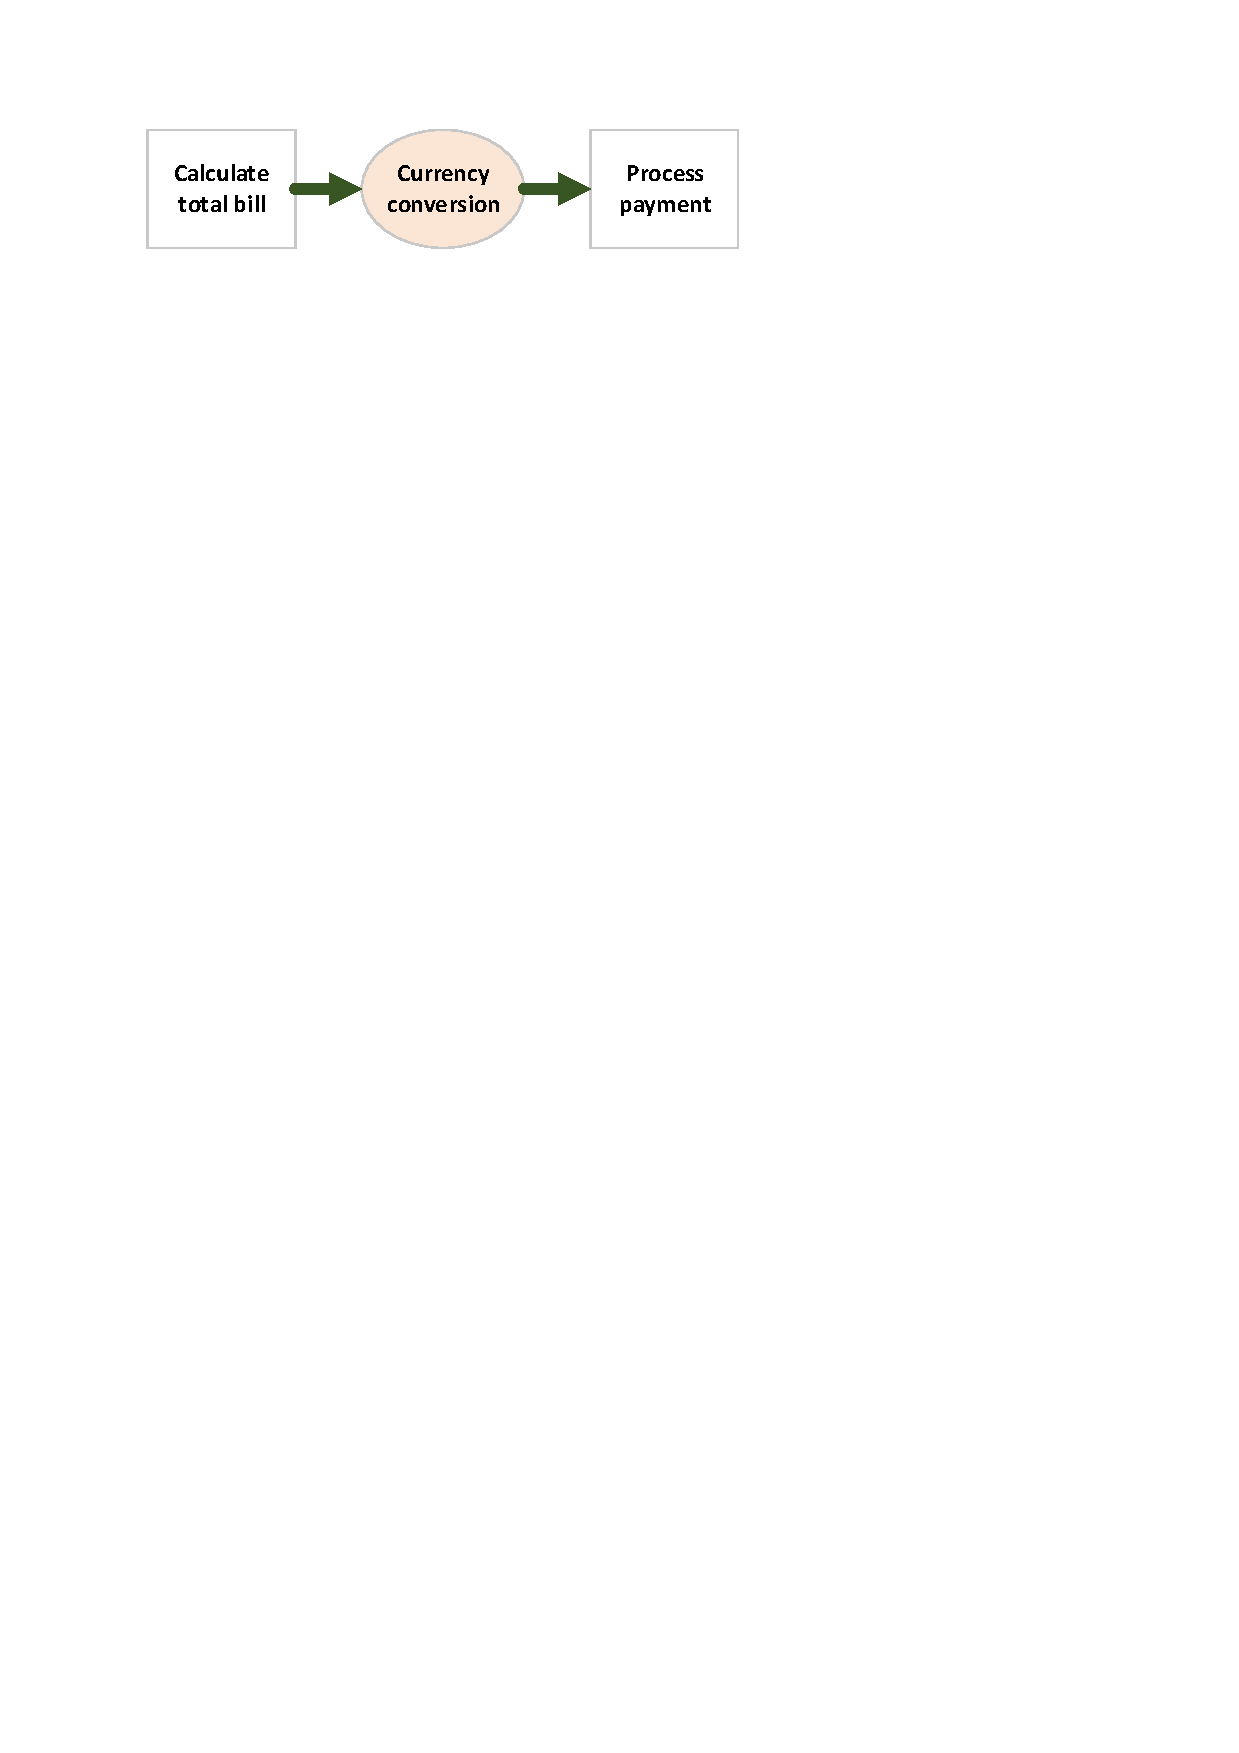
\includegraphics[width=7cm]{currency_example.pdf}}
\vfill
\begin{block}{Web service}
A functionality module that provides operations accessible over the network via a standard communication protocol.
\end{block}
\end{frame}

\note{
\begin{itemize}
 \item As the web becomes more and more pervasive, so does the concept of Service-Oriented Architecture.
 \item The idea in SOA is to organise business processes and data into independent modules which can then be reused in applicactions as needed.
 \item  For example, an e-commerce website may need to perform currency conversion depending on the location of its current customer, and so it uses an already existing currency conversion module.
 \item The basic components in SOA are services, which are functionality modules accessible over the network. In this example, currency conversion is a Web service.
\end{itemize}
}

%------------------------------------------------

\begin{frame}
\frametitle{Web Service Composition}
The combination of Web services to achieve a more complex task. Fully automated scenario:
\vfill
\centerline{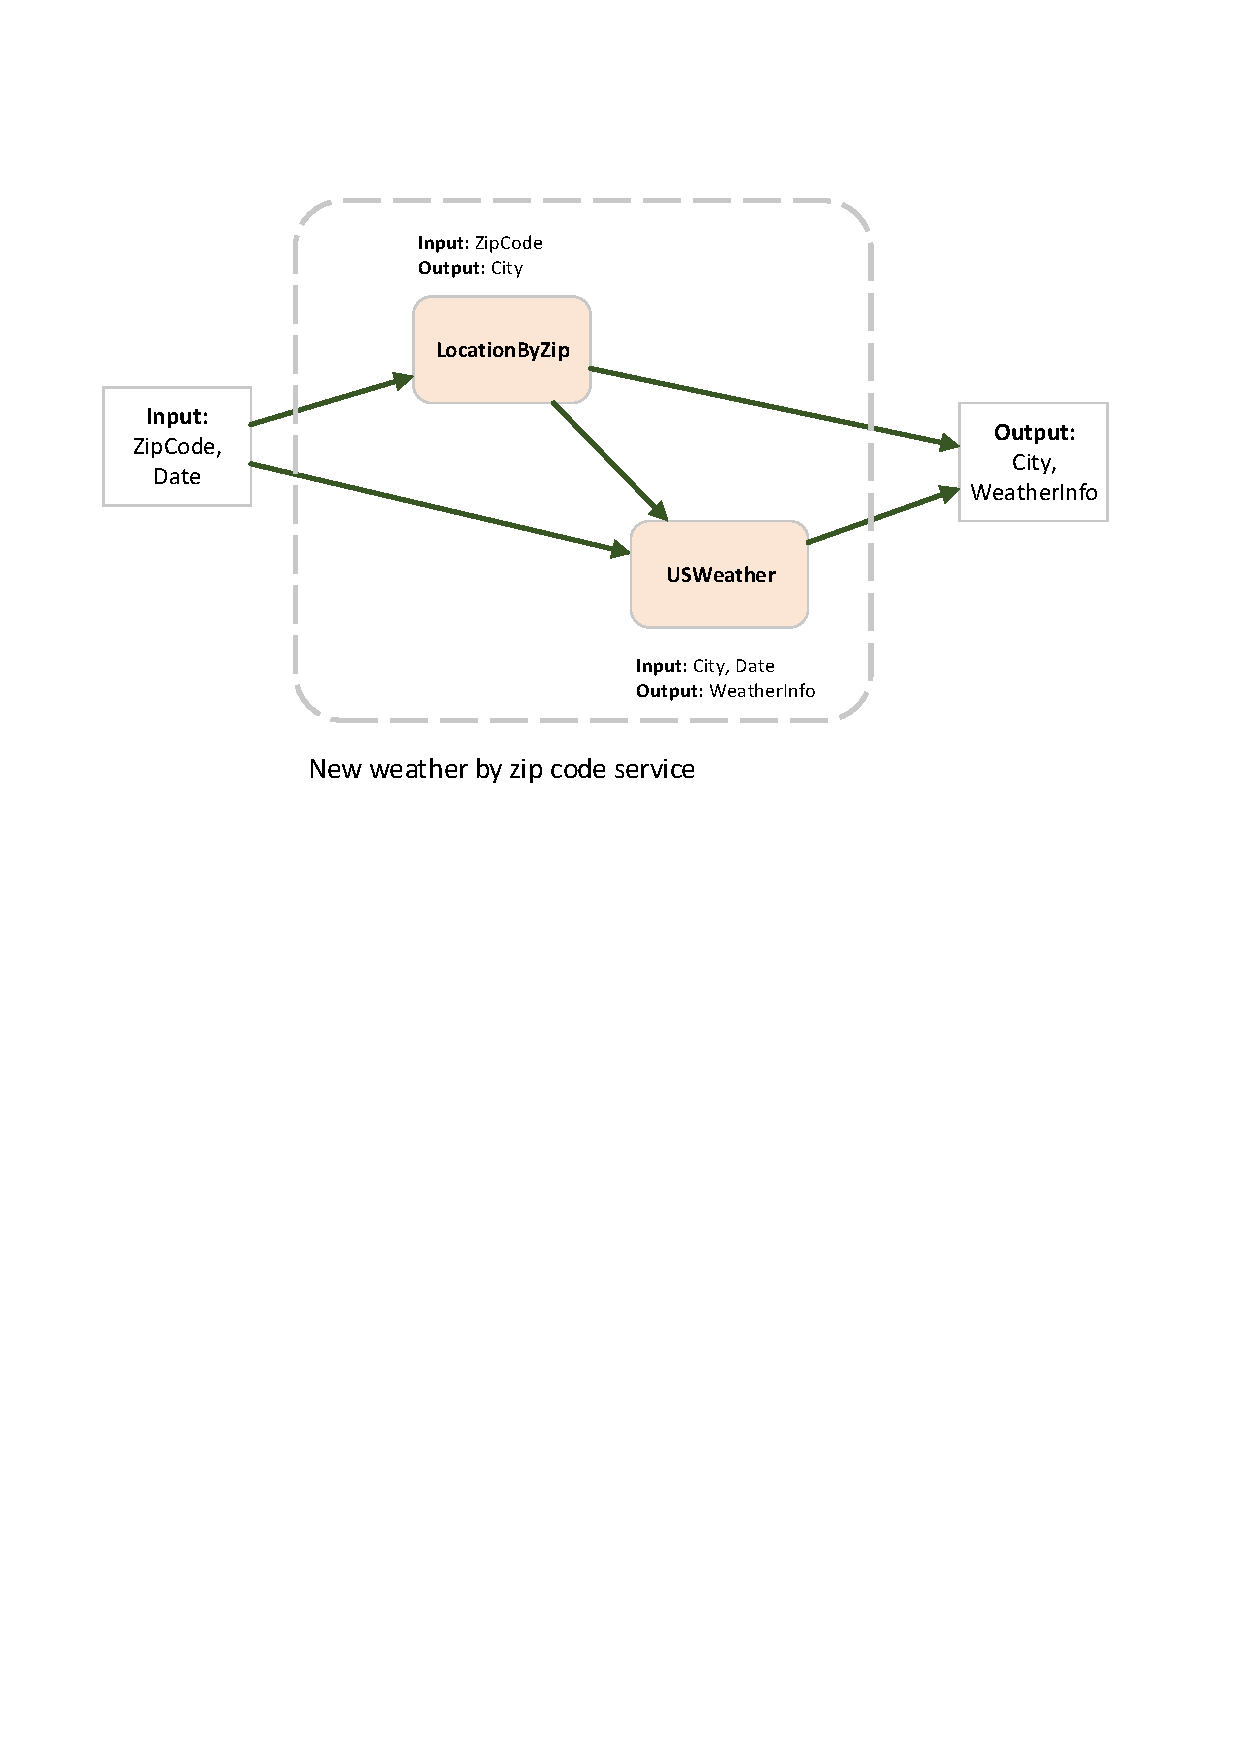
\includegraphics[width=10cm]{fully_automated_example.pdf}}
\end{frame}

\note{
\begin{itemize}
 \item The combination of multiple modular Web services in order to achieve a single, more complex task is known as Web service composition.
 \item Developing a system capable of creating such compositions in a fully automated manner is one of the holy grails of the field.
 \item With full automation, new services can be created simply by specifying the inputs the new service should require and the outputs it should produce, and the resulting composition is treated as a black box.
 \item For example, imagine we need to create a service that provides the weather forecast of a location based on its ZIP code. An automated composition system could identify and connect two different services, one that identifies a city based on a ZIP code and another that uses the city and date information to produce the forecast.
\end{itemize}
}

%------------------------------------------------

\begin{frame}
\frametitle{Composition Dimensions}
\begin{enumerate}
\item \textbf{Functional correctness:} Service inputs and outputs must be properly linked (e.g. \textcolor{blue}{$FourDigitNumber \rightarrow ZipCode$}, but not \textcolor{blue}{$FourDigitNumber \rightarrow City$}).
\vfill
\item \textbf{Conditional constraints:} Condition leading to multiple possible execution paths (e.g. if \textcolor{blue}{$City$} is a \textcolor{blue}{$NewZealandCity$}, produce \textcolor{blue}{$WindForecast$} instead of \textcolor{blue}{$GeneralForecast$}).
\vfill
\item \textbf{Quality of Service (QoS):} The overall quality of the composition (e.g. \textcolor{blue}{lowest execution time}, \textcolor{blue}{lowest cost}).
\end{enumerate}
\end{frame}

\note{
\begin{itemize}
 \item The complexity of Web service composition lies in the number of different dimensions it must consider at the same time.
 \item In the first dimension, we must ensure that services have their inputs and outputs properly linked. For example, a service that produces a four-digit number should be able to feed its output to the input of a service that accepts a zip code, however a four-digit number should not be accepted as a city name.
 \item In the second dimension, we must consider conditions that lead to different execution paths. For example, if a city is located in New Zealand, we would like a wind-only forecast as opposed to a general one.
 \item In the third dimension, we must produce compositions with the best possible quality attributes. For example, we would like it to have the lowest possible execution time as well as the lowest possible financial cost.
\end{itemize}

}

%------------------------------------------------

\begin{frame}
\frametitle{Existing Approaches}
{
\setbeamercolor{block title}{bg=red!40, fg=black}
\begin{block}{\textbf{AI Planning}}
Build a solution service by service.\\
Dimensions: \textit{Functional correctness, conditional constraints.}
\end{block}
}

\vfill
{
\setbeamercolor{block title}{bg=green!40, fg=black}
\begin{block}{\textbf{Evolutionary Computation (EC)}}
Improve population of solutions over multiple generations.\\
Dimensions: \textit{Functional correctness, QoS.}
\end{block}
}

\vfill
{
\setbeamercolor{block title}{bg=cyan!40, fg=black}
\begin{block}{\textbf{Hybrid Approaches}}
Combine AI planning and EC ideas.\\
Dimensions: \textit{Functional correctness, QoS.}
\end{block}
}
\end{frame}

\note{
\begin{itemize}
 \item Several techniques have been proposed to address the composition problem, however these approaches only account for at most two dimensions at once.
 \item In AI planning, a solution is built step by step, in each step adding a service and verifying the overall state of the composition. This approach typically verifies functional correctness and conditional constraints, but not the overall QoS.
 \item In evolutionary computation, a population of solutions is created and improved over multiple generations. This approach typically verifies functional correctness and optimises the overall QoS, but does not address conditional constraints.
 \item Hybrid approaches combine elements of AI planning and EC, making it easier to check the functional correctness and at the same time optimise the overall QoS. However, this approach also fails to address conditional constraints.
\end{itemize}
}

%------------------------------------------------

\begin{frame}
\frametitle{Goal}
To propose a Genetic Programming (GP) composition approach that simultaneously considers all dimensions.
\vfill

\begin{columns}[c]
\column{0.3\textwidth}
\begin{enumerate}
 \item Trees preserve functional correctness
 \vfill
 \item Conditions encoded in trees
 \vfill
 \item Optimisation performed on QoS
\end{enumerate}

\column{0.5\textwidth}
\centerline{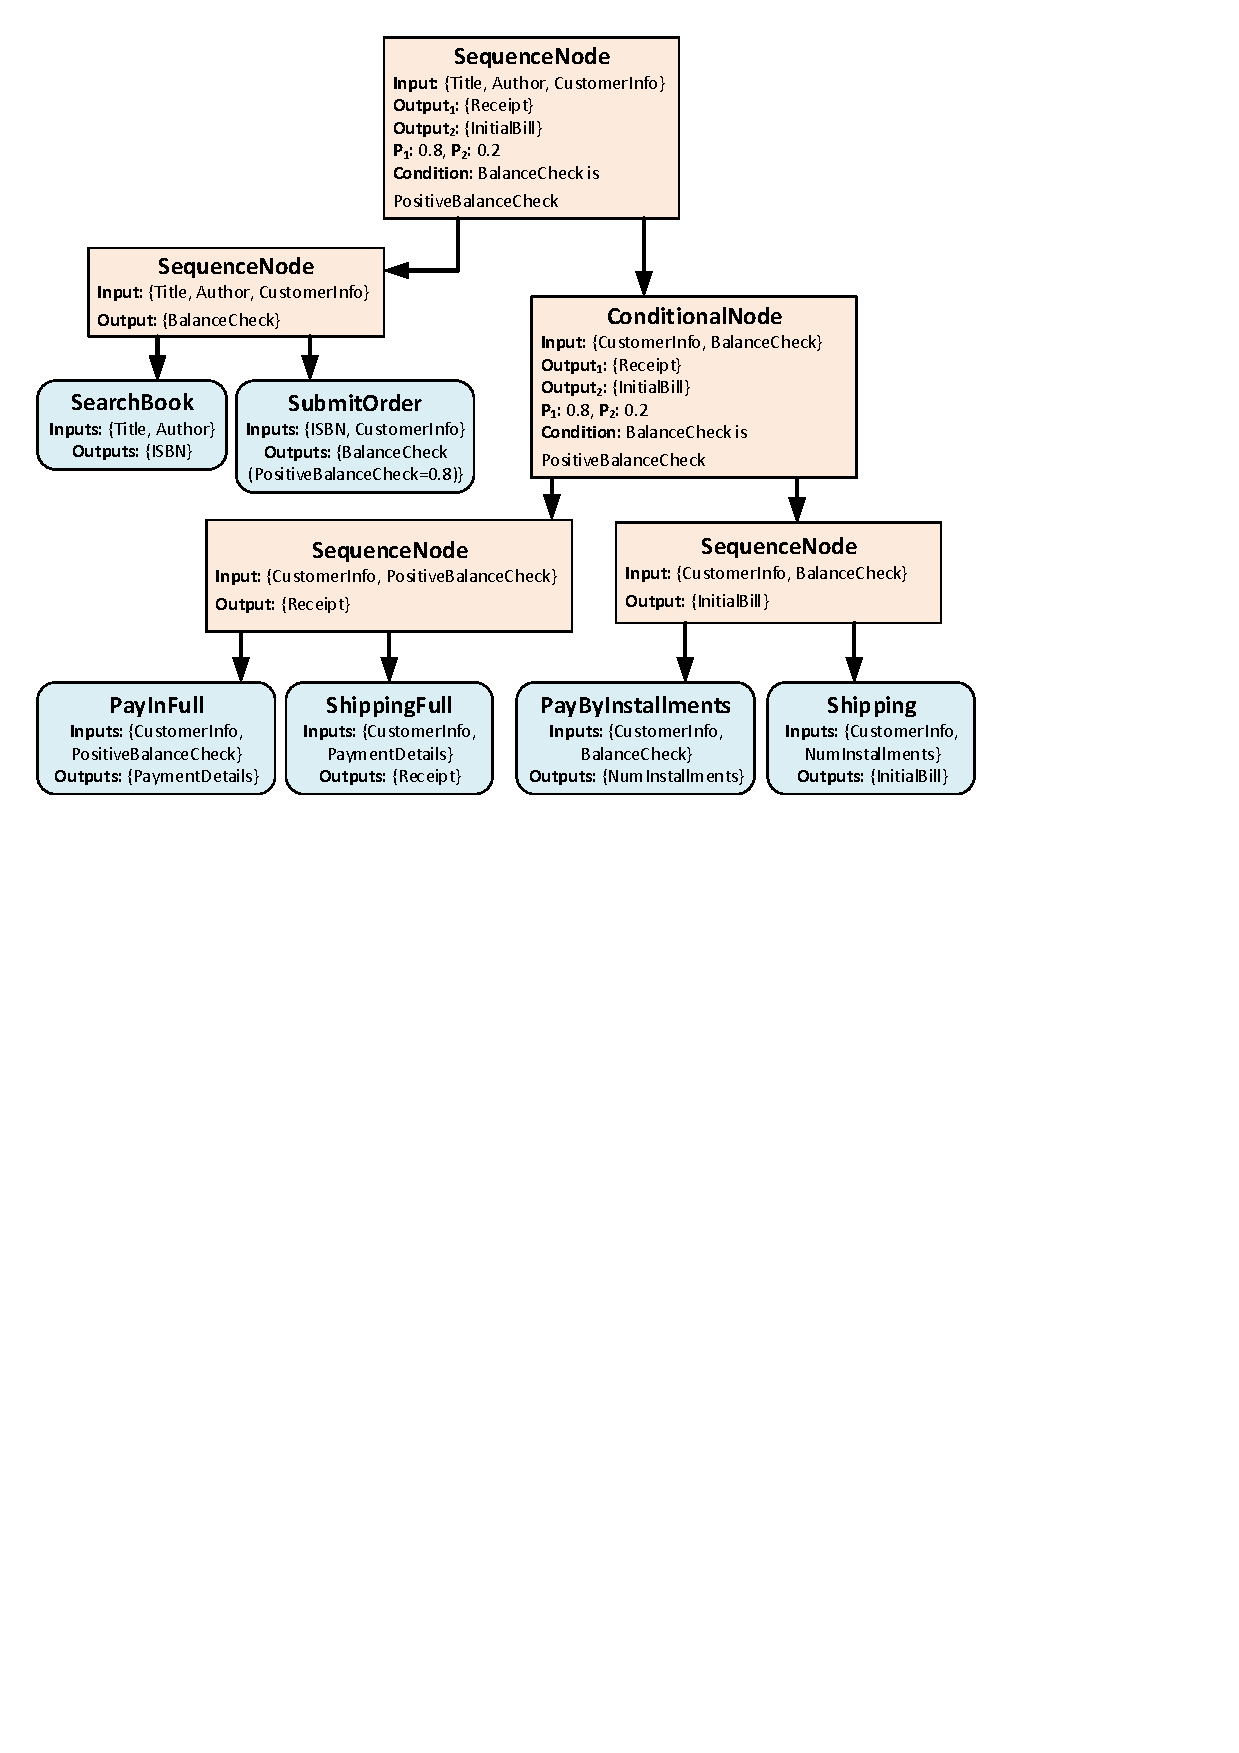
\includegraphics[width=6cm]{tree.pdf}}
\end{columns}

\end{frame}

\note{
\begin{itemize}
 \item Given these limitations, the objective of the approach proposed in this paper is to address these three dimensions simultaneously by using genetic programming.
 \item The functional correctness dimension is addressed by restricting the way in which services are linked to each other in each solution tree.
 \item Conditional constraints are addressed by including a conditional nodes as possible nodes in the tree representation.
 \item The Quality of Service dimension is addressed by using a fitness function that optimises solutions on quality attributes.
 \item Let's understand these in more detail.
\end{itemize}

}

%------------------------------------------------
\section{GP Approach}
\subsection{}
%------------------------------------------------

\begin{frame}
 \frametitle{Candidate Representation}
 \centerline{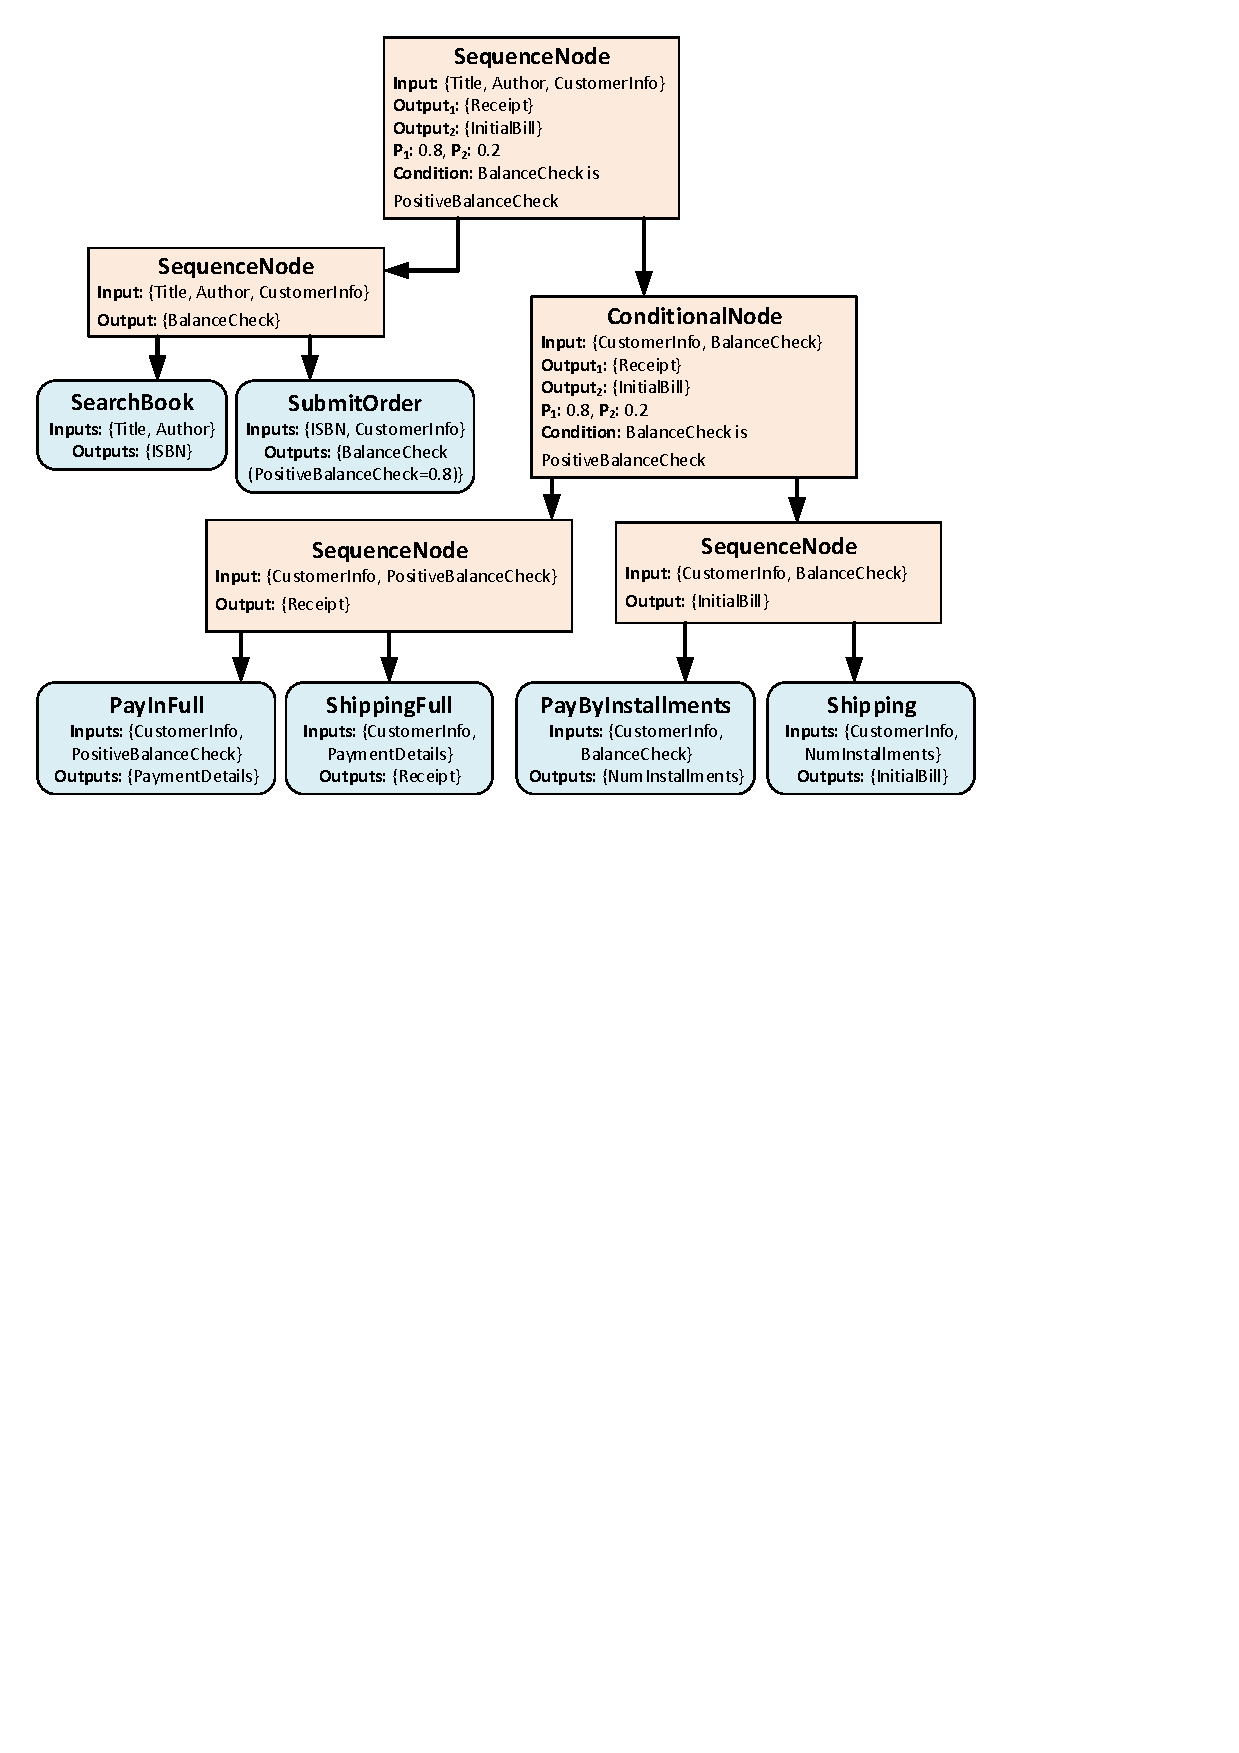
\includegraphics[width=6cm]{tree.pdf}}
\end{frame}


\begin{frame}
\frametitle{Population Initialisation}
An algorithm is used to create a candidate in graph format, and then translate it into a tree representation.

\vfill

\begin{columns}
\column{7cm}
\hspace{1cm}
%\centerline{
\fbox{
\scalebox{.40}{
\begin{algorithm*}[H]
 \setlength\hsize{0.9\linewidth}
 \SetKwInOut{Input}{Input}\SetKwInOut{Output}{Output}
 \SetKwFunction{createGraph}{createGraph}\SetKwFunction{toTree}{toTree}
 \LinesNumbered
 \SetNlSty{}{}{:}
 \Input{$I$, $O_1$, $O_2$, $C$, $P$}
 \Output{candidate tree $T$}
 \eIf{$O_2 \neq \emptyset$}{
  $G_1 \leftarrow \createGraph(I \cup C.if, O_1)$\;
  $G_2 \leftarrow \createGraph(I \cup C.else, O_2)$\;
  $T_1 \leftarrow \toTree(G_1.input)$\;
  $T_2 \leftarrow \toTree(G_2.input)$\;
  $T_3 \leftarrow$ new $ConditionalNode$($C$)\;
  $T_3.leftChild \leftarrow T_1$\;
  $T_3.rightChild \leftarrow T_2$\;
  \eIf{$C \sqsubseteq I$}{
    $T_3.prob \leftarrow P$\;
    \KwRet $T_3$\;
  }{
    $G_4 \leftarrow \createGraph(I, C.else)$\;
    $T_4 \leftarrow \toTree(G_4.input)$\;
    $T_3.prob \leftarrow T_4.final.P$\;
    $T \leftarrow$ new $SequenceNode$()\;
    $T.leftChild \leftarrow T_4$\;
    $T.rightChild \leftarrow T_3$\;
    \KwRet $T$\;
  }
 }{
  $G \leftarrow \createGraph(I, O_1)$\;
  $T \leftarrow \toTree(G.input)$\;
  \KwRet $T$\;
 }
% \vspace{2mm}
% \caption{\footnotesize Generating a new candidate tree or a mutated subtree.}
%\label{generation}
\end{algorithm*}
}}%}

\column{4cm}
\hspace{-2cm}
\centerline{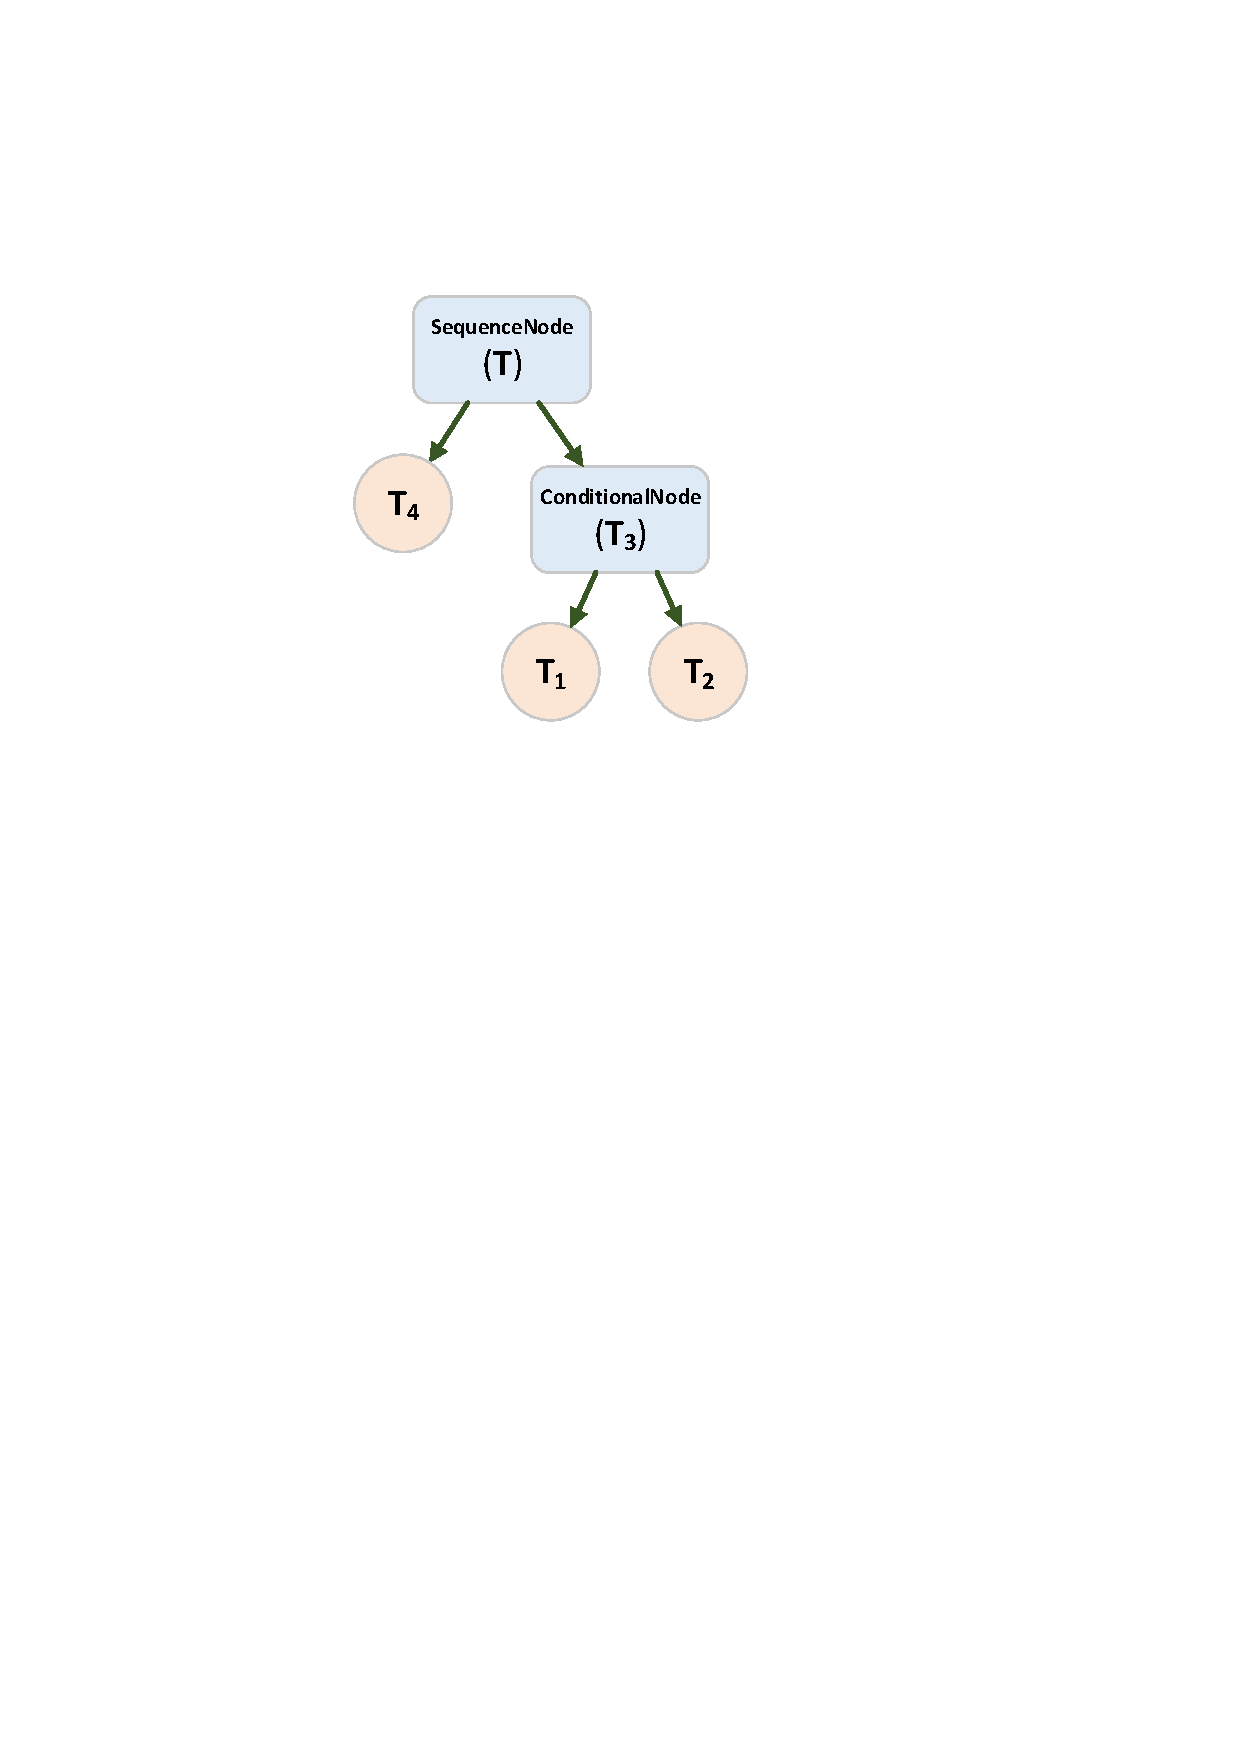
\includegraphics[width=4cm]{algorithm_tree.pdf}}
\end{columns}
\end{frame}

%------------------------------------------------

\begin{frame}
\frametitle{Mutation and Crossover}

\end{frame}

%------------------------------------------------

\begin{frame}
\frametitle{Fitness Function}

\end{frame}

%------------------------------------------------
\section{Experiments}
\subsection{}
%------------------------------------------------

\begin{frame}[fragile] % Need to use the fragile option when verbatim is used in the slide
\frametitle{Verbatim}
\begin{example}[Theorem Slide Code]
\begin{verbatim}
\begin{frame}
\frametitle{Theorem}
\begin{theorem}[Mass--energy equivalence]
$E = mc^2$
\end{theorem}
\end{frame}\end{verbatim}
\end{example}
\end{frame}

%------------------------------------------------

\begin{frame}
\frametitle{Figure}
Uncomment the code on this slide to include your own image from the same directory as the template .TeX file.
%\begin{figure}
%\includegraphics[width=0.8\linewidth]{test}
%\end{figure}
\end{frame}

%------------------------------------------------

\begin{frame}[fragile] % Need to use the fragile option when verbatim is used in the slide
\frametitle{Citation}
An example of the \verb|\cite| command to cite within the presentation:\\~

This statement requires citation \cite{p1}.
\end{frame}

%------------------------------------------------
\section{Conclusions}
\subsection{}
%------------------------------------------------

\begin{frame}
\frametitle{References}
\footnotesize{
\begin{thebibliography}{99} % Beamer does not support BibTeX so references must be inserted manually as below
\bibitem[Smith, 2012]{p1} John Smith (2012)
\newblock Title of the publication
\newblock \emph{Journal Name} 12(3), 45 -- 678.
\end{thebibliography}
}
\end{frame}

%------------------------------------------------

\begin{frame}
\Large
\centerline{Thank you!}
\medskip
\centerline{Questions\textcolor{red}{\textbf{?}}}
\end{frame}

%----------------------------------------------------------------------------------------

\end{document} 